% =====================================================================
%  Template de Resumo — XXX Seminário de Iniciação Científica da UEFS
%  Semana Nacional de Ciência e Tecnologia — 2026
%
%  Compilar:  pdflatex resumo_semic2026.tex
%  Requer:    cabecalho.png  (bloco do cabeçalho institucional com logos)
%
%  As medidas abaixo foram extraídas do PDF de referência com pdftotext
%  -bbox-layout, não estimadas:
%    margem esquerda/direita = 85,1 / 85,8 pt  -> 3,0 cm
%    primeira linha de tinta = 70,3 pt do topo
%    largura do cabeçalho    = 308,0 pt na linha "XXX SEMINÁRIO..."
% =====================================================================
\documentclass[12pt,a4paper]{article}

% O PDF de referência usa Times New Roman real (pdffonts: TimesNewRomanPSMT).
% Com lualatex/xelatex usamos a Liberation Serif, que é metricamente idêntica
% à Times New Roman e portanto produz as MESMAS quebras de linha. Com pdflatex
% cai no mathptmx, visualmente igual mas com métrica ligeiramente diferente,
% o que desloca algumas quebras.
%
%   lualatex resumo_semic2026.tex   <- recomendado, reproduz a referência
%   pdflatex resumo_semic2026.tex   <- funciona, com pequenas diferenças
\usepackage{iftex}
\ifPDFTeX
  \usepackage[T1]{fontenc}
  \usepackage[utf8]{inputenc}
  \usepackage{mathptmx}
\else
  \usepackage{fontspec}
  \setmainfont{Liberation Serif}  % substitua por "Times New Roman" se instalada
\fi
\usepackage[brazilian]{babel}

% top=53,5 pt posiciona a PRIMEIRA TINTA da imagem do cabeçalho em ~62 pt,
% ajustado empiricamente (referência: 70,3 pt, PNG tem margem interna <8 pt).
\usepackage{geometry}
\geometry{a4paper, left=3cm, right=3cm, top=53.5pt, bottom=2.5cm}

\usepackage{graphicx}
\usepackage{booktabs}
\usepackage{array}
\usepackage{titlesec}
\usepackage{caption}
\usepackage[hidelinks]{hyperref}

% Permite quebra de \texttt{} em sublinhados — sem isso identificadores
% longos como teleop_twist_keyboard provocam overfull hbox.
\usepackage[htt]{hyphenat}

% Citação numérica estilo IEEE via bibtex (referencias.bib). Diferente de
% um thebibliography manual, só aparecem aqui as entradas efetivamente
% citadas com \cite{} no texto — nenhuma curadoria manual é necessária.
% Compilar: pdflatex -> bibtex resumo_semic2026 -> pdflatex -> pdflatex.
\usepackage[numbers]{natbib}
\bibliographystyle{unsrtnat}

% Seções sem numeração, negrito, alinhadas à esquerda. O texto não é
% convertido para maiúsculas: alguns títulos do modelo misturam caixa,
% como "RESULTADOS E/OU DISCUSSÃO (ou Análise e discussão dos resultados)".
\setcounter{secnumdepth}{0}
\titleformat{\section}{\normalfont\bfseries}{}{0pt}{}
\titlespacing*{\section}{0pt}{14.9pt plus 2pt minus 2pt}{1.3pt}

% Tabela: legenda acima, centralizada, separador ponto.
% Figura:  legenda abaixo, justificada, menor, rótulo em negrito, dois-pontos.
\captionsetup[table]{labelsep=period, justification=centering,
                     font=normalsize, skip=4pt}
\captionsetup[figure]{labelsep=colon, justification=justified,
                      font=small, labelfont=bf, skip=6pt}

% Entrelinha de 15,87 pt, medido no PDF de referência. O padrão do 12 pt é
% 14,45 pt, o que acumularia ~50 pt de defasagem ao longo da página.
\linespread{1.098}

\setlength{\parindent}{0pt}
% Espaçamento entre parágrafos: ~meia linha, acompanhando o modelo da UEFS.
\setlength{\parskip}{6pt plus 1pt minus 1pt}

% O ambiente center injeta ~10 pt acima e abaixo (\topsep + \parskip), o que
% empurra todo o bloco de título/autores para baixo. Esta versão não injeta
% nada, deixando o espaçamento inteiramente sob controle dos \vspace.
\newenvironment{bloco}
  {\setlength{\topsep}{0pt}\setlength{\partopsep}{0pt}\begin{center}}
  {\end{center}}

\begin{document}
\pagestyle{empty}   % o modelo não numera as páginas

% ---------------------------------------------------------------------
% CABEÇALHO INSTITUCIONAL (imagem: logos + texto em Arial)
% 328 pt reproduz a largura medida no PDF de referência. O \makebox evita
% o espaço vertical extra que o ambiente center introduziria.
% ---------------------------------------------------------------------
\noindent\makebox[\textwidth][c]{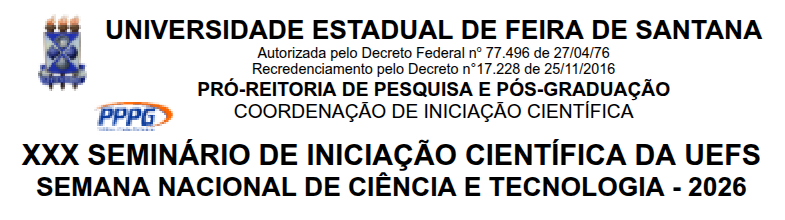
\includegraphics[width=328pt]{cabecalho.png}}

\vspace{4.6pt}

% ---------------------------------------------------------------------
% TÍTULO
% Com o \linespread global o título já sai com os 15,9 pt da referência.
% ---------------------------------------------------------------------
\begin{bloco}
    \textbf{Interface de Controle Mioelétrico Baseado no Sensor Myo Armband para\\
    Teleoperação de Robôs}
\end{bloco}

\vspace{17.8pt}

% ---------------------------------------------------------------------
% AUTORES
% ---------------------------------------------------------------------
\begin{bloco}
    \underline{\textbf{Yasmin Cordeiro de Souza Meira}}\textsuperscript{1};
    \textbf{Anfranserai Morais Dias}\textsuperscript{2}
\end{bloco}

\vspace{0.6pt}

% As linhas de afiliação são mais largas que a mancha de texto no original
% (começam em 62,4 pt, à esquerda da margem de 85,1 pt). O \makebox permite
% esse transbordo sem aviso de overfull. O corpo 9,5 reproduz a largura
% medida na referência; o entrelinha de 11,9 pt, o espaçamento entre as duas.
\noindent\makebox[\textwidth][c]{%
  \begin{minipage}{1.14\textwidth}
    \centering
    \fontsize{9.5}{10.84}\selectfont
    1.Yasmin Cordeiro de Souza Meira, PIBIC/FAPESB, ENGENHARIA DE COMPUTAÇÃO, e-mail: ymeira@ecomp.uefs.br\\
    2.Anfranserai Morais Dias, DEPARTAMENTO DE TECNOLOGIA, e-mail: amdias@uefs.br
  \end{minipage}}

\vspace{20.2pt}

\begin{bloco}
    \textbf{PALAVRAS-CHAVE:} uma; duas; três
\end{bloco}

\vspace{1pt}

% ---------------------------------------------------------------------
\section{INTRODUÇÃO}

A teleoperação em ambientes de difícil acesso tem impulsionado a transição de
controles manuais limitados (como joysticks), cuja restrição de graus de
liberdade dificulta o comando intuitivo de plataformas com múltiplas
articulações~\cite{li2019intuitive}, para interfaces mais intuitivas capazes
de capturar movimentos naturais do operador. Nesse cenário, a eletromiografia
de superfície (sEMG) ganhou destaque por sua robustez a variações de
iluminação e a outras limitações físicas que afetam sensores
visuais~\cite{sultana2023systematic}, especialmente por meio de dispositivos
acessíveis como o Myo Armband, braçadeira de baixo custo que integra sensores
de sEMG e uma unidade de medida inercial (IMU)~\cite{visconti2018technical}.
Embora a literatura já demonstre a eficácia dessa tecnologia no controle de
robôs com rodas~\cite{sathiyanarayanan2015controlling,morais2016application},
resta uma lacuna no uso dessas interfaces em plataformas de complexidade
superior, como robôs com patas, nas quais a latência fim a fim do canal de
comando impacta diretamente a estabilidade da
marcha~\cite{siegwart2011introduction,risiglione2021passivity}.

Para endereçar essa lacuna, este trabalho apresenta o desenvolvimento e a
caracterização de uma interface de teleoperação mioelétrica para o robô
quadrúpede SH3 [descrição breve], sob restrições estritas de tempo real. A
solução baseia-se em uma arquitetura de três camadas (computador do operador,
Raspberry Pi e microcontrolador embarcado) que desacopla a aquisição de
sinais, a classificação de cinco gestos (repouso, flexão, extensão, desvio
ulnar e desvio radial) e a atuação nos servomotores, combinando o
\textit{framework} micro-ROS 2 a estratégias de mitigação de latência no
\textit{firmware}.

Os resultados experimentais demonstraram que a interface proposta alcançou uma
acurácia de classificação de gestos de [INSERIR \%] e uma latência fim a fim
média de [INSERIR ms]; além disso, as análises qualitativas de trajetória confirmaram que
o controle intuitivo permitiu manter a estabilidade dinâmica da marcha do
robô durante a locomoção. O restante deste artigo está organizado como segue:
a Seção~2 detalha a metodologia, a arquitetura de hardware/software e os
algoritmos de filtragem; a Seção~3 apresenta e discute os resultados de
latência e desempenho; e a Seção~4 consolida as conclusões e aponta direções
para trabalhos futuros.

% ---------------------------------------------------------------------
\section{METODOLOGIA}

\subsection*{2.1 Visão geral da arquitetura}

O sistema é organizado em três camadas, cujo fluxo de dados é ilustrado na
Figura~\ref{fig:arquitetura}. Na primeira camada, a braçadeira Myo Armband
adquire dados de movimento e de atividade muscular do operador e os
transmite a um computador central. Esse computador executa o
pré-processamento dos sinais e um classificador de gestos, inspirado na
implementação de Caffagni~\cite{caffagni2023myo}, e publica, via ROS 2, as
velocidades linear e angular correspondentes ao gesto reconhecido. Na
segunda camada, uma Raspberry Pi hospeda o agente micro-ROS 2 e retransmite
ao microcontrolador as mensagens recebidas da camada anterior por Wi-Fi
(ROS~2 DDS); para isso, configurou-se uma subrede dedicada que permitiu a
propagação dos comandos do ROS~2 e o reconhecimento mútuo dos tópicos e nós
do computador operador e da Raspberry Pi. Na terceira camada, um Raspberry
Pi Pico (RP2350) recebe essas velocidades e as converte em comandos de
posição, enviados em alta frequência à placa controladora SSC-32 através do
protocolo UART, responsável pelo acionamento dos servomotores. Em paralelo,
o Pico lê os sensores embarcados: fluxo óptico PMW3901, infravermelho
SharpIR, sonar HC-SR04 e IMU MPU9250/MPU6500.

\begin{figure}[htbp]
\centering
% Substitua pelo diagrama de blocos definitivo:
% \includegraphics[width=0.9\textwidth]{arquitetura.png}
\framebox[0.9\textwidth][c]{\rule{0pt}{4cm}\textit{diagrama de blocos da arquitetura em três camadas (a inserir)}}
\caption{Arquitetura em três camadas. As setas tracejadas indicam os pontos
$t_0$ e $t_1$ usados para medir a latência fim a fim.}
\label{fig:arquitetura}
\end{figure}

\subsection*{2.2 Aquisição, pré-processamento e classificação}
\label{sec:aquisicao-classificacao}

Os sinais do operador são adquiridos pela braçadeira Myo Armband, que
combina oito canais de eletromiografia de superfície (sEMG) e uma
unidade de medida inercial (IMU) com acelerômetro e giroscópio
triaxiais. O dispositivo foi escolhido por seu custo-benefício e por
sua crescente popularidade na comunidade científica ~\cite{mendez2017evaluation}. No sistema,
braçadeira conecta-se diretamente ao computador por Bluetooth, com o
EMG em modo bruto, sem filtragem ou retificação pelo dispositivo, e os
sinais são processados em tempo real.

No pré-processamento, as leituras da IMU são apenas convertidas para o
Sistema Internacional (m/s\textsuperscript{2} e rad/s), garantindo
compatibilidade com o ROS~2, e alimentam duas verificações sucessivas
que decidem se o EMG deve ser processado. A primeira estima a
inclinação (\textit{pitch}) do antebraço a partir da direção da
gravidade medida pelo acelerômetro, suavizada por uma média móvel
exponencial, e só autoriza o prosseguimento quando o antebraço está
próximo da horizontal, dentro de uma tolerância angular em torno do
alvo (Tabela~\ref{tab:parametros}). Essa restrição de postura busca
reduzir a variabilidade do sinal mioelétrico associada à posição do
membro, efeito documentado por Fougner \textit{et
al.}~\cite{fougner2011limb}, que mostram sua degradação da
classificação e propõem medir a posição do membro com acelerômetros. A
segunda verificação aplica, sobre o mesmo sinal de IMU, o detector de
parada SHOE, formulado por Skog \textit{et al.}~\cite{skog2010zero} e
aqui reaproveitado para reconhecer quando o antebraço está parado.
Assim, o EMG só é processado quando o antebraço está na orientação correta e
em movimento; caso contrário, suas amostras são descartadas.

Satisfeitas as duas condições, o EMG é acumulado em janelas de 30
amostras (150~ms a 200~Hz), valor no limite inferior da faixa de 150 a
250~ms que Smith \textit{et al.}~\cite{smith2011window} identificaram
como ótima no sistema que avaliaram, no qual janelas maiores reduzem o
erro de classificação, mas aumentam o atraso do controlador. Para cada
canal, extraem-se quatro descritores no domínio do tempo: valor
absoluto médio (MAV), comprimento de forma de onda (WL), número de
cruzamentos por zero (ZC) e número de trocas de sinal da derivada
(SSC)~\cite{hudgins1993new}. O vetor resultante é normalizado por
reescala linear e enviado ao classificador, e, após cada decisão, um
intervalo refratário de 20 amostras (100~ms) suprime novas decisões.

% Figura 1 (Seção 2.1): sugere-se destacar nela o trecho
% IMU -> postura -> movimento -> EMG -> SVM -> velocidades.

\begin{table}[htbp]
\centering
\caption{Parâmetros do pré-processamento e da classificação. Canais e
taxas são especificações do dispositivo; os demais valores foram
definidos empiricamente ou pelo protocolo de coleta.}
\label{tab:parametros}
\small
\begin{tabular}{@{}lc@{}}
\toprule
\textbf{Parâmetro} & \textbf{Valor} \\
\midrule
Canais de sEMG & 8 \\
Taxa de envio do EMG & [CONFIRMAR] \\
Taxa de envio da IMU & [CONFIRMAR] \\
Alvo de \textit{pitch} & 0$^\circ$ \\
Tolerância de \textit{pitch} & $\pm 30^\circ$ \\
Constante da média exponencial ($\alpha$) & 0,1 \\
Janela do detector de movimento & 20 amostras \\
Limiar do detector de movimento ($\gamma$) & 45 \\
Janela de EMG & 30 amostras (150~ms) \\
Intervalo refratário & 20 amostras (100~ms) \\
Classes de gesto & 5 \\
Janelas coletadas por classe & 50 \\
Divisão treino/teste & 80\,\%~/~20\,\% (estratificada) \\
\bottomrule
\end{tabular}
\end{table}

Por fim, o vetor de características é classificado por uma máquina de vetores de suporte (SVM) com núcleo radial (RBF)~\cite{cortes1995svm}, escolhida pelo baixo custo computacional de inferência, compatível com a operação em tempo real sem aceleração dedicada. Para treiná-la, construiu-se uma base própria, com um único participante em uma única sessão, composta por cinquenta janelas para cada uma das cinco classes de gesto, registradas com o gesto sustentado e divididas em 80,\% para treino e 20,\% para teste. Em operação, cada gesto reconhecido pelo modelo treinado é convertido em velocidades linear e angular, publicadas via ROS~2 para a camada intermediária do sistema (Seção~\ref{sec:camada-intermediaria}).

\subsection*{2.3 Camada intermediária}

A Raspberry Pi recebe \texttt{/cmd\_vel} por rede local (Wi-Fi) e hospeda o
agente XRCE-DDS que serializa as mensagens ao RP2350 por USB CDC
(\textit{Communications Device Class}). Essa escolha dispensa conversor
USB-serial — removendo o \textit{jitter} e a latência de um chip
FTDI/CP210x do caminho — e usa o mesmo cabo para alimentar o microcontrolador.

\subsection*{2.4 \textit{Firmware} embarcado (RP2350)}

O laço principal do \textit{firmware} alterna o atendimento do executor
micro-ROS (\texttt{rclc\_executor\_spin\_some}, orçamento de 10~ms por
iteração) com a rotina de marcha, que gera a trajetória nominal dos servos
em função do \texttt{/cmd\_vel} corrente e a transmite à SSC-32 por UART. As
leituras dos sensores são desacopladas desse laço por meio das seguintes
estratégias de mitigação de latência: (i) \textit{Direct Memory Access}
(DMA) nas transações do PMW3901 (SPI) e da MPU9250/MPU6500 (I$^2$C),
evitando que o núcleo responsável pela marcha seja bloqueado em operações de
entrada e saída; (ii) temporização dos ciclos periódicos de amostragem por
\textit{hardware alarms} do RP2350, eliminando laços de espera e reduzindo o
\textit{jitter} de amostragem; (iii) medição do pulso de eco do HC-SR04 por
interrupção de borda em GPIO (\textit{General Purpose Input/Output}),
dispensando leitura bloqueante; e (iv) um \textit{watchdog} sobre as
transações DMA que aborta e rearma a cadeia quando o escravo não confirma a
transferência em 5~ms, impedindo que uma falha isolada paralise o laço.

\subsection*{2.5 Protocolo experimental}

A coleta da base de treino do classificador e a divisão treino/teste já
foram descritas na Seção 2.2. Esta subseção cobre apenas o protocolo de
medição de latência e de avaliação qualitativa das trajetórias.

A latência fim a fim é medida por \textit{timestamps} em dois pontos:
$t_0$ = instante da decisão do classificador no computador operador, e
$t_1$ = instante do recebimento do \texttt{/cmd\_vel} correspondente no
\texttt{cmd\_vel\_callback} do RP2350; o par é propagado como campo adicional
na própria mensagem para dispensar sincronização externa de relógios. São
realizadas [PREENCHER: número de repetições] medidas com o robô
[PREENCHER: parado em bancada / em marcha], das quais se reportam média e
desvio padrão. Como condição de referência, repete-se o protocolo substituindo
o pacote Myo pelo \texttt{teleop\_twist\_keyboard}, executado no mesmo
computador operador e publicando \texttt{/cmd\_vel} sobre a mesma rede
Wi-Fi — isolando, portanto, apenas o segmento \textit{aquisição + classificação}
com o restante do caminho idêntico ao do protocolo principal. A coerência
qualitativa das trajetórias é avaliada visualmente comparando-se as leituras
publicadas pelos sensores embarcados (fluxo óptico, distância IR e sonar) ao
comportamento observado do robô durante a locomoção.

% ---------------------------------------------------------------------
\section{RESULTADOS E/OU DISCUSSÃO (ou Análise e discussão dos resultados)}

Apresentação e discussão dos resultados obtidos. Ilustrações como figuras,
gráficos, fluxogramas e tabelas deverão ser incluídas no corpo do texto. Figuras
e tabelas devem estar centralizadas entre as margens do texto. Figuras, fotos e
gráficos devem ser apresentados com tamanho e detalhes suficientes. Evitar
tabelas extensas, privilegiando-se dados médios, adequar tamanho ao espaço útil
do papel, e suas legendas devem ser auto-explicativas. A numeração da ilustração
deve ser sucessiva em algarismos arábicos (Tabela 1; Figura 1, por exemplo).

\vspace{8pt}

\begin{table}[htbp]
\centering
\caption{Principais características anatômicas das folhas de oito espécies de
\textit{Pouteria} Aublet (Sapotaceae) ocorrentes no estado da Bahia}
\label{tab:exemplo}

{\small
\begin{tabular}{@{}l*{8}{c}@{}}
\toprule
 & \multicolumn{8}{c}{\textbf{Espécies}} \\
\cmidrule(l){2-9}
\textbf{Caracteres} & \textbf{1} & \textbf{2} & \textbf{3} & \textbf{4}
                    & \textbf{5} & \textbf{6} & \textbf{7} & \textbf{8} \\
\midrule
Ornamentação cuticular na epiderme adaxial & + & - & + & - & - & - & + & - \\
Paredes anticlinais retas                  & + & - & - & - & + & + & - & - \\
Paredes anticlinais sinuosas               & - & + & + & + & - & - & + & + \\
Estômato anomocítico                       & - & - & - & - & + & - & + & - \\
Estômato anisocítico                       & + & + & + & + & - & + & - & + \\
Mesofilo dorsiventral                      & + & + & + & - & + & + & + & + \\
Mesofilo isobilateral                      & - & - & - & + & - & - & - & - \\
Número de camadas da epiderme              & 1 & 1 & 1 & 1 & 2 & 1 & 1 & 3 \\
Número de camadas de parênquima paliçádico & 2 & 2 & 1 & 1 & 3 & 2 & 2 & 3 \\
Laticíferos                                & + & + & + & + & + & + & + & + \\
Tricomas                                   & - & + & + & + & - & + & + & - \\
\bottomrule
\end{tabular}}

\vspace{4pt}
{\footnotesize
Legenda: 1. \textit{Pouteria andarahiensis} T.D.Penn., 2. \textit{P. caimito}
(Ruiz \& Pavón) Radlk., 3. \textit{P. gardneri} (Mart. \& Miq.) Baehni,
4. \textit{P. gardneriana} (A.DC.) Radlk., 5. \textit{P. grandiflora} (A.DC.)
Baehni, 6. \textit{P. ramiflora} (Mart.) Radlk., 7. \textit{P. torta} (Mart.)
Radlk., 8. \textit{P. venosa} (Mart.) Baehni. (+) = presente; (-) = ausente.}
\end{table}

\begin{figure}[htbp]
\centering
% Substitua pelo seu arquivo de imagem:
% \includegraphics[width=0.75\textwidth]{figura1.png}
\framebox[0.75\textwidth][c]{\rule{0pt}{5cm}\textit{espaço reservado para a figura}}
\caption{Tipos polínicos observados nas amostras coletadas na Chapada
Diamantina-BA. \textbf{A} - Acanthaceae (\textit{Anisacanthus}); B -
Apocynaceae (\textit{Prestonia}); C-; Arecaceae. D - Asteraceae;
E - Bignoniaceae (\textit{Zeyheria}); F - Campanulaceae (\textit{Centropogun});
G - Lamiaceae (\textit{Hyptis}); H - Malvaceae (\textit{Helicteres});
I - Malvaceae (\textit{Pavonia}) J - Mimosa \textit{pudica}
K - Myrtaceae (\textit{Eucalyptus}) L -- Poaceae.}
\label{fig:exemplo}
\end{figure}

As citações bibliográficas no texto deverão seguir os seguintes modelos: Quate
(1965); (Quate, 1965); Erwin \& Sott (1980); Guimarães \textit{et al.} (1983). Os
artigos devem ser citados em ordem cronológica. Todas as referências mencionadas
no texto devem ser arroladas no final do trabalho. O último nome dos autores deve
ser digitado em MAIÚSCULAS (ver modelo abaixo). Periódicos deverão ser abreviados
de acordo com o \textit{World List of Scientific Periodicals} ou como indicado
pelo próprio periódico ou, em caso de dúvida, buscar no site:
\url{http://library.caltech.edu/reference/abbreviations}. A forma de citações das
referências deve estar de acordo com os exemplos aqui apresentados.

% ---------------------------------------------------------------------
\section{CONSIDERAÇÕES FINAIS (ou Conclusão)}

O(s) último(s) parágrafo(s) dos resultados e discussão deve(m) trazer as
conclusões sumarizadas na forma de texto corrido.

% ---------------------------------------------------------------------
% Bibliografia via bibtex (referencias.bib): só entram aqui as referências
% com \cite{} usado em algum ponto do texto. Remover um \cite não deixa
% entrada órfã — ela simplesmente some da lista na próxima compilação.
\renewcommand{\refname}{REFERÊNCIAS}
\bibliography{referencias}

\end{document}
